\section{The Perceptron}
\label{sec:perceptron}
When researchers developed the first machine learning models, they often used ideas based closely on our understanding of the brain. One such model, inspired by the biological neuron, is the perceptron \cite{McCulloch1943115}.

Like its biological counterpart, the perceptron receives information and produces an output. More specifically, it accepts $n$ input values $x_1, \ldots, x_n$ and calculates a corresponding output value $\hat{y} \in \{-1, 1\}$ by computing
\begin{equation}\label{eq:perceptron1}
	\hat{y} = \sign\left (\sum_{i=1}^{n} w_ix_i\right ),
\end{equation}
where the weights $w_i$ are the parameters of the model, and $\sign(x)$ is defined as
\begin{equation}
\sign(x) = \begin{cases} 1 & \text{if }x > 0
							\\-1 & \text{if }x \leq 0.
\end{cases}
\end{equation}
By representing the input values and weights as vectors $\bm{x}$ and $\bm{w}$, we can rewrite Eq. \eqref{eq:perceptron1} as
\begin{equation}
\hat{y} = \sign(\bm{w}^\top\bm{x}).
\end{equation}
For a visual representation of this model, see Fig. \ref{fig:perceptron}. 
\begin{figure}
	\begin{center}
		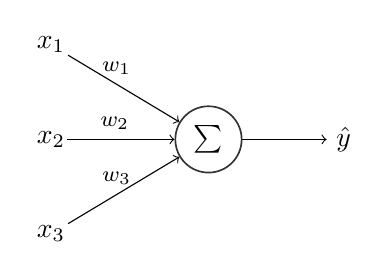
\begin{tikzpicture}
	\tikzstyle{neuron} = [circle,draw=black!80,semithick,minimum size=20pt]
	% input layer
	\foreach \i in {1,...,3}
		\node (input\i) at (0, -\i*1.2) {$x_\i$};
	% perceptron
	\node[neuron] (perceptron) at (2, -2*1.2) {$\sum$};
	% connections
	\foreach \i in {1,...,3}
		\draw[->, shorten <= -.1cm] (input\i) -- node[pos=.4,above]{\footnotesize{$w_\i$}} (perceptron);
	% output
	\draw[->] (perceptron) -- node[above]{$\sign$}(3.5, -2*1.2) node[right]{$\hat{y}$};
\end{tikzpicture}
	\end{center}
	\caption{An illustration of the perceptron model. In this example, the perceptron accepts three inputs $x_1, x_2, x_3$, has the parameters $w_1, w_2, w_3$, and computes $\hat{y} = \sign(w_1x_1 + w_2x_2 + w_3x_3).$}
	\label{fig:perceptron}
\end{figure}

Perceptron models can be used to solve binary classification problems. In this scenario, we are given a list of $m$ training examples $\mathbb{X} = (\bm{x}^{(1)}, \ldots, \bm{x}^{(m)})$ and their corresponding binary labels $\mathbb{Y}$, and wish to predict the most probable label for an unseen vector $\bm{x} \notin \mathbb{X}$.

For example, the vectors $\bm{x}^{(i)}$ might describe features of an email using a \emph{bag-of-words} representation. That is, we define a fixed vocabulary, and the \nth{j} entry in the vector $\bm{x}^{(i)}$ specifies how often the \nth{j} word of the vocabulary occurs in the particular email represented by $\bm{x}^{(i)}$. The corresponding label $y^{(i)} = 1$ then might signify that the email is a legitimate email, whereas a value of $y^{(i)} = -1$ might label the email as spam.

In the beginning, the weights are randomly initialized and the model thus makes arbitrary predictions. During the process of \emph{training} the perceptron, we iteratively adjust the weights in order to improve the prediction accuracy on the training set.

One common method of training is the perceptron learning algorithm proposed by Rosenblatt \cite{Rosenblatt1958386}, which we will not cover in this paper, since it is not directly applicable to neural networks. An in depth explanation can be found in Ref. \cite[Ch.\,8,\,pp.\,265-267]{DBLP:books/lib/Murphy12}.

A major shortcoming of the perceptron is that it can only learn to classify linearly separable data \cite{DBLP:books/daglib/0066902}. For example, the \textsc{xor} function, where 
\begin{equation}
\text{\textsc{xor}}(\bm{x}) = 
\begin{cases} 0 & \text{if }\bm{x} = [0,0] \lor \bm{x} = [1,1] 
			\\1 & \text{if }\bm{x} = [1,0] \lor \bm{x} = [0,1],
\end{cases}
\end{equation}
cannot be learned with the perceptron, since there exists no linear function that perfectly partitions the data into the two classes $0$ and $1$. The discovery of these limitations has greatly reduced interest in the field of biological learning, until more sophisticated models, such as neural networks, were developed \cite[Ch.\,1,\,pp.\,12-18]{DBLP:books/daglib/0040158}.